% Chapter 12, Section 3

\section{Speech Recognition and Synthesis \difficultyInline{beginner}}
\label{sec:speech-applications}

\subsection{Automatic Speech Recognition (ASR)}

Convert speech to text using acoustic front-ends and sequence models; self-supervised pretraining (e.g., wav2vec) reduces labeled data needs \textcite{Prince2023}.
\begin{itemize}
    \item Virtual assistants (Siri, Alexa, Google Assistant)
    \item Transcription services
    \item Voice commands
\end{itemize}

\textbf{Architectures:} CTC-based models, Listen-Attend-Spell, Transducer models, wav2vec.

\begin{figure}[h]
  \centering
  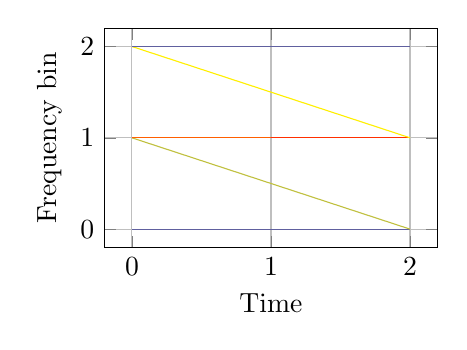
\begin{tikzpicture}
    \begin{axis}[
      width=0.48\textwidth,height=0.36\textwidth,
      xlabel={Time}, ylabel={Frequency bin}, grid=both]
      \addplot[mesh,draw=none,shader=interp,point meta=explicit] coordinates{ (0,0) [0.1] (1,0) [0.2] (2,0) [0.1]
        (0,1) [0.3] (1,1) [0.5] (2,1) [0.4]
        (0,2) [0.1] (1,2) [0.2] (2,2) [0.1] };
    \end{axis}
  \end{tikzpicture}
  \caption{Schematic spectrogram input for ASR.}
  \label{fig:asr-spec}
\end{figure}

\subsection{Text-to-Speech (TTS)}

Generate natural-sounding speech with neural vocoders; evaluate with MOS and intelligibility measures.
\begin{itemize}
    \item WaveNet, Tacotron
    \item Voice cloning
    \item Accessibility tools
\end{itemize}

\subsection{Speaker Recognition}

Identify speakers:
\begin{itemize}
    \item Voice biometrics
    \item Speaker diarization (who spoke when)
\end{itemize}

\subsection{Historical context and references}

End-to-end ASR and neural TTS displaced classical pipelines by learning representations directly from data. Self-supervised audio pretraining further improved robustness \textcite{Prince2023}.

